% ------------------------------------------------------------------------ %
% !TEX encoding = UTF-8
% !TEX TS-program = pdflatex
% !TEX root = ../Project.tex
% !TEX spellcheck = en-EN
% ------------------------------------------------------------------------ %
%
% ------------------------------------------------------------------------ %
% 	CHAPTER TITLE
% ------------------------------------------------------------------------ %
%
\chapter{Algorithm Design}
%
\label{cap:algorithmdesign}
%
%
In this section we show the idea behind the algorithms structure of the core functions of the system. We choose to elaborate on the processes concerning the creation of a new event, the update of the planned trips of all user's events, the trip planning, the calculation of the travel time for shared means of transport (due to the fact that it is not directly obtainable from Google Maps API) and the users's dynamic events scheduling, which are the main objectives of the system. 
After the user inputs the data of a new event, the system will first run the overlapping check algorithm, which will than run the trips update algorithm to keep them up to date. This second process is of great importance, and will be run every time there is a change in preferences, events or trips, in addition of a daily update.  
The main block of the update algorithm is the trip planning one, checking the feasibility of the trips and suggesting the best way to reach an event. This one will be run more frequently than usual when it is almost time to start a trip. 
We decided to show a flow chart with processes, serving as code description to ease the understanding, due to the more schematic  form in blocks. The code is written in a pseudo java inspired on the probable class structure of the system.
The objective is to show the reader the logic under the decision precesses of our sistem, made to be as practical and human-like as possible when proposing the beat travel solution.
\vspace{10mm}
%
% ------------------------------------------------------------------------ %
\begin{center}
\thispagestyle{empty}
\makebox[\textwidth][c]{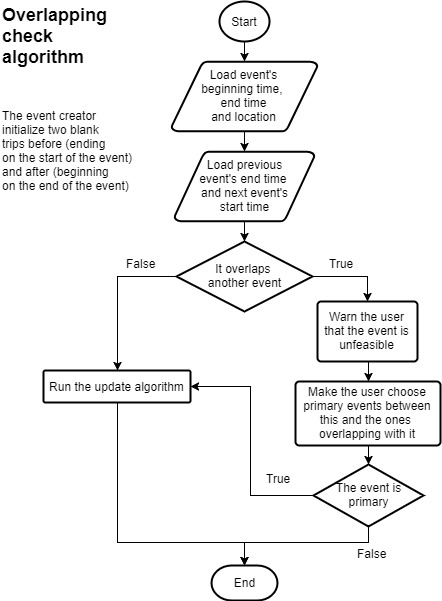
\includegraphics[width=1.08\textwidth]{MainMatter/images/algo/1overlap_check_algo}}
\captionof{figure}{Overlap check algorithm}
\end{center}
\lstinputlisting[language=Java]{MainMatter/srccode/overlapping_algo.java}
%
\begin{center}
\thispagestyle{empty}
\makebox[\textwidth][c]{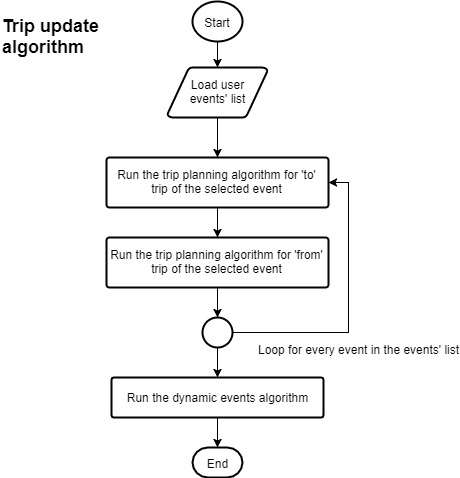
\includegraphics[width=1\textwidth]{MainMatter/images/algo/2trip_update_algo}}
\captionof{figure}{Trip update algorithm}
\end{center}
\lstinputlisting[language=Java]{MainMatter/srccode/trip_update.java}
%
\begin{center}
\thispagestyle{empty}
\makebox[\textwidth][c]{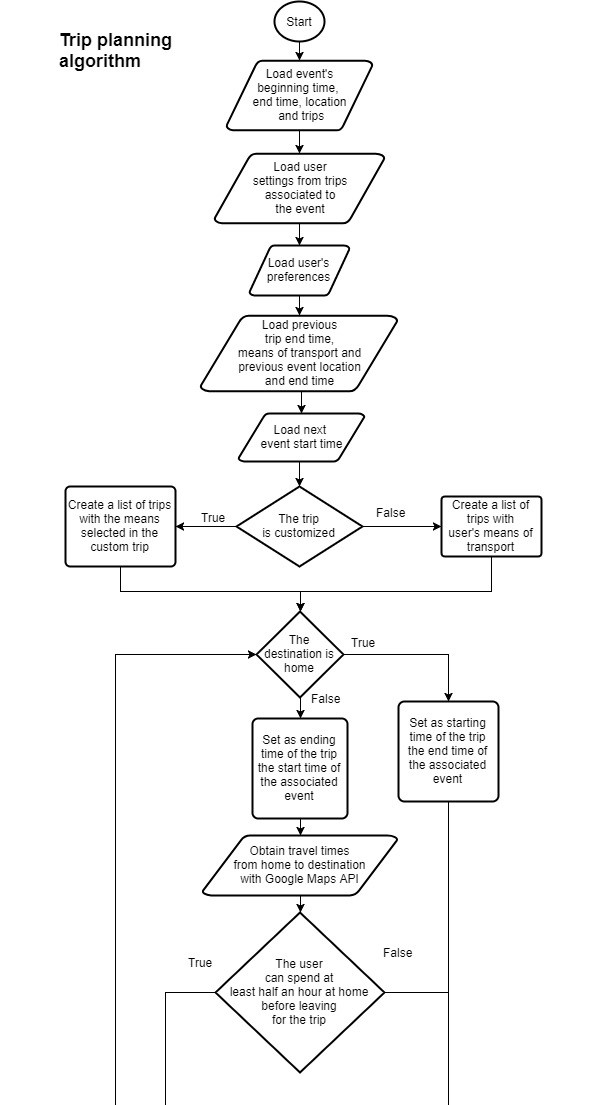
\includegraphics[width=0.8\textwidth]{MainMatter/images/algo/3trip_planning1}}
\captionof{figure}{Trip planning algorithm part 1}
\end{center}
%
\begin{center}
\thispagestyle{empty}
\makebox[\textwidth][c]{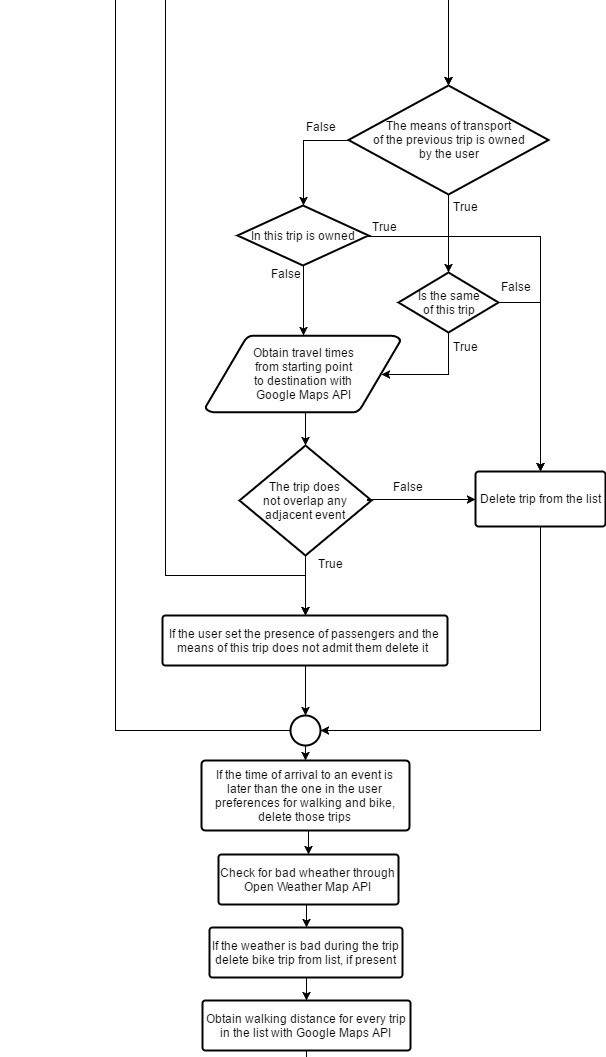
\includegraphics[width=0.78\textwidth]{MainMatter/images/algo/3trip_planning2}}
\captionof{figure}{Trip planning algorithm part 2}
\end{center}
%
\begin{center}
\thispagestyle{empty}
\makebox[\textwidth][c]{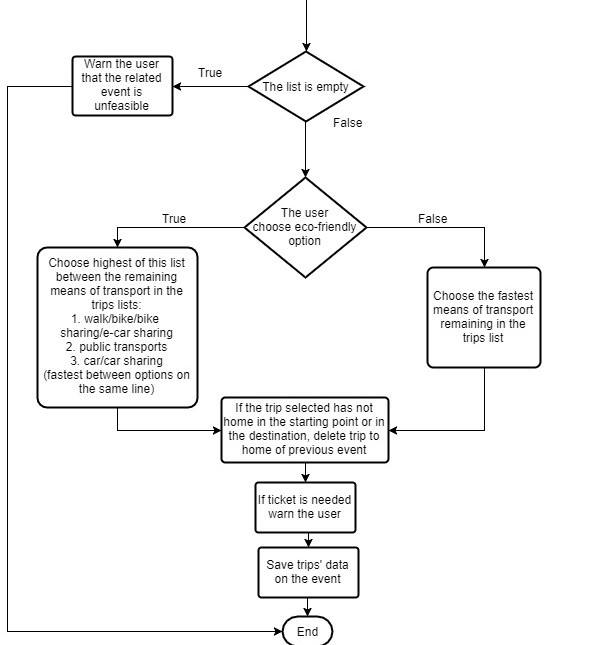
\includegraphics[width=1\textwidth]{MainMatter/images/algo/3trip_planning3}}
\captionof{figure}{Trip planning algorithm part 3}
\end{center}
\pagebreak
\lstinputlisting[language=Java]{MainMatter/srccode/trip_planning_algo.java}
%
\begin{center}
\thispagestyle{empty}
\makebox[\textwidth][c]{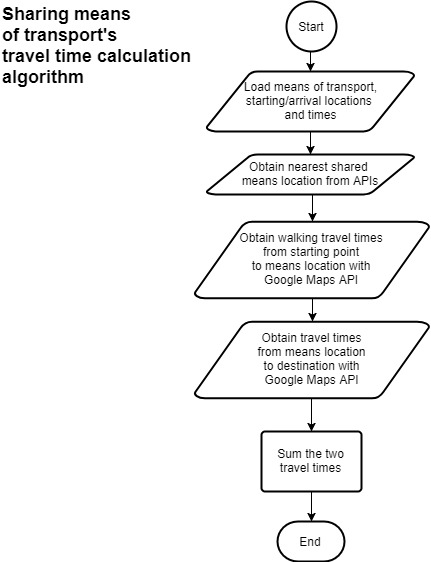
\includegraphics[width=1.1\textwidth]{MainMatter/images/algo/4sharing_algo}}
\captionof{figure}{Sharing means of transport algorithm}
\end{center}
%
\begin{center}
\thispagestyle{empty}
\makebox[\textwidth][c]{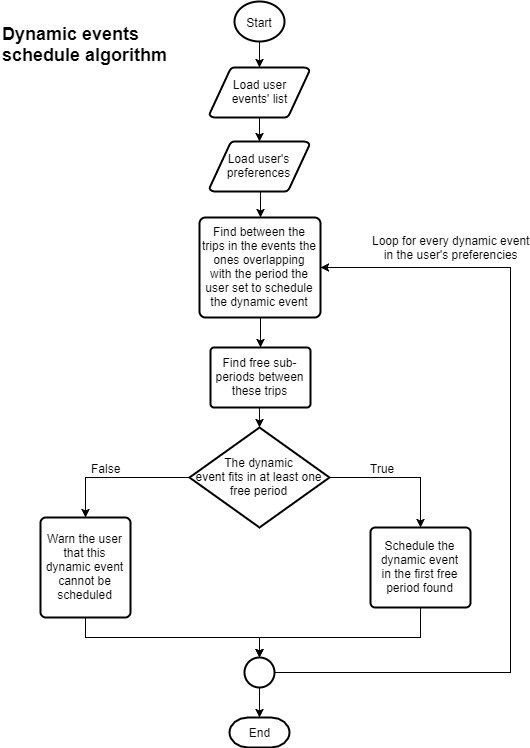
\includegraphics[width=1.04\textwidth]{MainMatter/images/algo/5dynamic_algo}}
\captionof{figure}{Dynamic event schedule algorithm}
\end{center}
\lstinputlisting[language=Java]{MainMatter/srccode/dynamic_events_algo.java}
%
% -----------------------------END------------------------------------- %
